\item Due segmenti AB ed AC sono sovrapposti come in figura. Se AB è lungo 4 cm ed AC è lungo 6 cm, che operazione fai per calcolare la lunghezza di BC?
\begin{figure}[h]
\centering
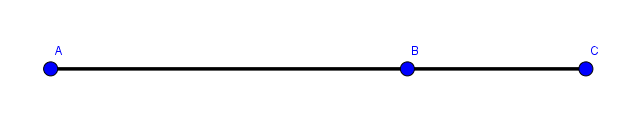
\includegraphics[width=13cm]{figure/somma_diff_segmenti.PNG}
\end{figure}
